\documentclass[twocolumn]{article}

\usepackage{ctex}
\usepackage{amsmath}
\usepackage{amsthm}
\usepackage[inline]{enumitem}
\usepackage{amsfonts}
\usepackage[margin=15mm]{geometry}
\usepackage[dvipdfm]{graphicx}
\DeclareGraphicsExtensions{.eps,.mps,.pdf,.jpg,.png}
\DeclareGraphicsRule{*}{eps}{*}{}
\graphicspath{{./jpg/}}

\begin{document}
\title{锥树最大内积搜索}
\maketitle

\begin{abstract}
在给定的集合中,高效地查找某个查询在欧氏距离和余弦相似度方面的最佳匹配这个问题已经有了广泛的研究。然而就我们所知,另一个与之紧密相关的问题,即在一般情况下,如何高效地查找内积方面最佳匹配的问题,却从未被探索过。本文将讨论这个问题,并与前面的那些问题进行比对。我们先提出一个通常意义上基于(单)树形数据结构的分支定界算法。随后,我们提出一个双树算法来应对多个查询的情况。我们给出的分支定界算法是建立在新的内积界限之上的。最后我们会给出一个新的数据结构,锥树,来提高双树的效率。我们用了各种应用中产生的大量数据集对这些算法进行了评估,在某些情况下,与暴力搜索的算法相比,查询速度提高了多达5个数量级。
\end{abstract}

\section*{分类和主题描述}
E.1 [数据结构]: 树; G.4 [数学软件]: 算法设计与分析; H.2.8 [数据库管理]: 数据库应用——数据挖掘; H.3.3 [信息存储与检索]: 信息查找与检索——查找过程
\section*{通用项}
算法, 设计
\section*{关键词}
定界度量树、锥树、双树分支定界

\section{介绍}
在这篇论文中,我们讨论的是在给定的点集内,如何高效地查找某个查询在内积相似度方面最佳匹配的问题。搜索效率的提高是我们主要的关注点。我们来正式考虑下面这个问题:

\paragraph{最大内积查询} 给定一个包含 $N$ 个点的集合 $S \subset \mathbb{R}^D$ 和一个查询 $q \in \mathbb{R}^D$,高效地找到一个点 $p \in S$ 使得
\begin{equation}
\langle q,p \rangle = \max_{r \in S}\langle q,r \rangle
\end{equation}

乍看之下,这个问题与很多已有文献做的工作十分类似。高效地查找在欧氏距离(或者更一般地 $L_p$)方面的最佳匹配,属于被人广泛研究的度量空间最近邻搜索问题\cite{9}。在文本挖掘和信息检索领域中,余弦相似性方面最佳匹配的高效检索已有相应的研究\cite{1}。不过在下一节我们会解释,最大内积搜索不仅与上述问题不同,而且更加困难。

\subsection{应用}
最大内积搜索的一个明显的应用,来自于诸如“Netflix Prize”\cite{22, 21, 2}这类推荐系统中所用的,已经大获成功的矩阵分解框架。矩阵分解使得可用的数据可以用“用户”向量和“商品”向量精确地表示出来(“商品”可以是音乐或者电影)。在这个背景下,用户对于商品的偏好就是对应的“用户”向量和“商品”向量的内积\footnote{偏好其实是用户和商品向量的内积加上一个偏移项,但是如果给用户向量添加一个1,给商品向量添加一个商品偏移量,那这个问题就退化成内积问题了。}。如果把用户当做查询,商品当做参考集合的话,对于用户推荐的检索就等同于最大内积搜索的问题。通常的做法是对商品进行线性扫描来查找最佳推荐。而高效的搜索算法会使得矩阵分解框架中的推荐检索可以向更大的系统中拓展。

常用的文档检索任务会使用余弦相似性来匹配文档。然而在特定的背景下\cite{11},文档会被表示成(不一定是标准化的)向量,向量间的内积就代表它们的相似度。在这样的情况下,除非向量被标准化成同样的长度,否则,要让用余弦相似度进行文档匹配的算法\cite{1}可扩展,可能会付出结果不准确的代价,毕竟内积和余弦相似性还是不一样的(我们会在第二节中进一步讨论这个问题)。

还有一个类似的问题就是最大核操作:给定一个点集$S$,一个查询$q$和一个核函数$\mathcal{K}(\cdot,\cdot)$,任务是,在集合$S$上找到一个点$p \in S$使得$\mathcal{K}(p,q)$最大。这个问题在机器学习中的最大后验推理\cite{20}和计算机视觉中的图像匹配\cite{23}中都得到了广泛的应用。如果核函数可以显式地表达成$\varphi(\cdot)$的形式,且满足$\mathcal{K}(p,q) = \langle \varphi(q), \varphi(r) \rangle$,并且集合$S$中的所有点和查询$q$都被转换到$\varphi$空间,那么这个问题就退化为最大内积搜索问题了。

\subsection{这篇论文}
在这篇论文中,我们提出两个基于树的分支定界算法以及一个新的数据结构来解决这个问题。
在第二节中,我们把这个问题和度量空间中一些更为常见的最近邻搜索问题,以及在余弦相似性方面的最佳匹配问题进行对比。
在第三节中,我们提出一个简单的分支定界算法,该算法使用的是已有的球树数据结构\cite{28}和一个新的界限。
在接下来一节(第四节)中,我们将处理同一个点集上多个查询的情况,并且提出基于双树的分支定界算法。
在第五节中,我们将展示一个新的数据结构,锥树,来对双树算法进行索引。这些结构利用了一个新的内积界限,这比传统的球树所能达到的界限更为严格。
在第六节中,我们将用不同的数据集对提出的这个算法进行评估。
第七节证明我们提出的这个算法可以被应用于最大核操作,而且使用的是一个通用的核函数而不需要显式地表示出$\varphi$-空间里的点。
在最后一节中,我们会给出我们的结论以及未来在这个问题上可能的研究方向。

\section{最大内积搜索}
现在已经有许多欧几里德度量空间中的最近邻搜索技术(见一些调查,如\cite{9})。大规模的针对余弦相似度测度\cite{1}的最佳匹配算法也已经建立起来,而他们的关注点大多都在文本数据上。(度量空间中的)最近邻搜索的问题也已经用广泛流行的局部敏感哈希(LSH)\cite{14,18}大致地解决了。LSH 已经被推广到其他形式的相似性函数(与把距离作为不相似函数相反),如余弦相似性\cite{7}\footnote{这里需要注意的是,Charikar 等人\cite{7}用的相似性函数不完全是余弦相似性,因为$p$和$q$两点的距离用的是$\theta$/$\pi$,其中$\theta$是两个点在原点处的夹角,使得相似性函数变为$\left(1-\frac{\theta}{\pi}\right)$。这个相似性函数可以和余弦相似度直接对应。}。
在满足特定条件的情况下,核函数上近似的最大核操作也可以通过LSH高效地解决。降维\cite{30}和双树算法\cite{20}也被用来高效地解决近似的最大核操作。

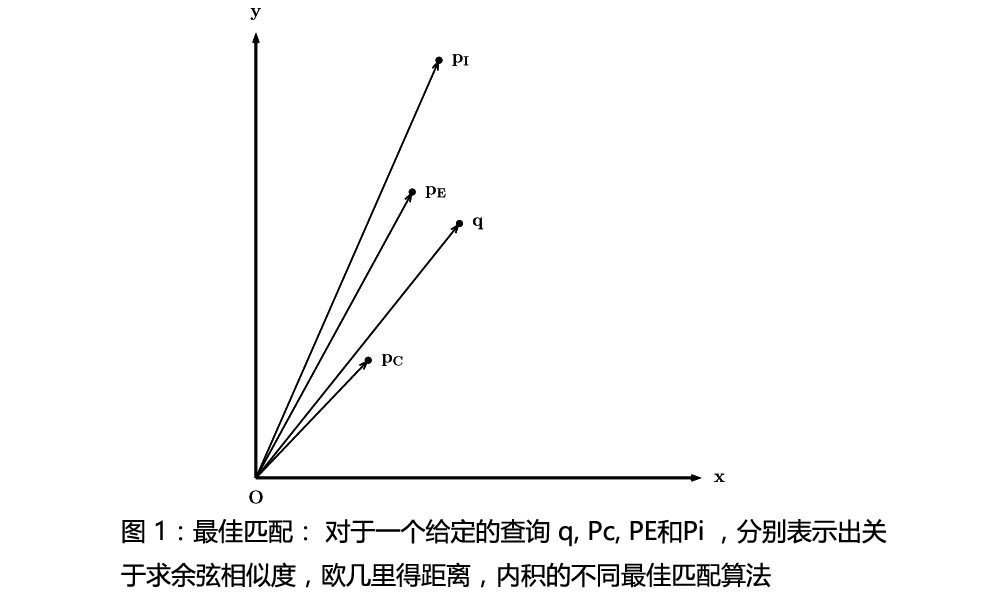
\includegraphics[width=300pt,clip,trim=30 0 0 0]{fig01.jpg}

\subsection{最大内积搜索和已有问题的不同}
这里我们解释下为什么最大内积搜索和其它已有的搜索问题都不太一样。因此用于解决那些问题的技术(如LSH)不能直接应用于这个问题。

\paragraph{欧式空间内的最近邻搜索}这涉及到对于一个查询$q$找到一个点$p \in S$使得:
\begin{align*}
p &= \arg \min_{r \in S}\|q - r\|^2_2 = \arg \max_{r \in S}\left(\langle q,r \rangle - \frac{\|r\|_2^2}{2}\right) \\
  &  \neq \arg \max_{r \in S} \langle q,r \rangle (\mathrm{unless}\ \|r\|_2^2 = k \forall r \in S).
\end{align*}
因此,如果$S$中所有点的范数被标准化为相同的长度,那么最大内积搜索等价于欧式度量空间中的最近邻搜索。然而没有这个限制的话,这两个问题就很可能会有截然不同的解(图 2)。

\paragraph{余弦相似度的最佳匹配}这构成了对于一个查询$q$找到一个点$p \in S$使得:
\begin{align*}
p &= \arg \max_{r \in S} \frac{\langle q,r \rangle}{\|q\|\|r\|} = \arg \max_{r \in S} \frac{\langle q,r \rangle}{\|r\|} \\
    &\neq \arg \max_{r \in S} \langle q,r \rangle (\mathrm{unless}\ \|r\|_2^2 = k \forall r \in S).
\end{align*}
仅当集合$S$中的所有点被标准化成相同的长度时,对于余弦相似性的最佳匹配给出的才是最大内积(见图 2 反例)。

\paragraph{局部敏感哈希}LSH已经被应用于各种相似性函数。LSH包括构造哈希函数,使得对于任意一对点$r,p \in S$,每个哈希函数$h$都满足下面这个条件:
\begin{equation}
\mathrm{Pr}[h(r) = h(p)] = \mathrm{sim}(r,p)
\end{equation}
其中$\mathrm{sim}(r,p) \in [0,1]$是我们关心的相似度函数。像我们这种情况,我们可以标准化我们的数据集使得$\forall r \in S, \|r\| \le 1$
\footnote{这里的标准化和前面提到的标准化是不同的,前面提到的标准化是将所有的点标准化为相同的长度。而在这里点的长度被标准化为远不等于1,但互不相等。},
并且假设所有的数据都在第一象限(这样没有内积会比零要小)。在这样的情况下,$\mathrm{sim}(r,p) = \langle r,p \rangle \in [0,1]$就是我们所关心的一个合法的相似度函数

我们知道,如果相似性函数存在对应的局部敏感哈希函数族,距离函数$\mathbf{d}(r,p) = 1 - \mathrm{sim}(r,p)$必须满足三角不等式(\cite{7}中的引理1)。
然而,距离函数$\mathbf{d}(r, p) = 1 - \langle r,p \rangle$并不满足三角不等式(甚至当所有点都被限制在第一象限时)
\footnote{反例:令点$x,y,z\in S$使得$\|x\|=\|y\|=\|z\|=1$,$x$和$y$,$y$和$z$,$z$和$x$之间的夹角分别为$\left(\frac{\pi}{4} - 0.1\right)$,$\frac{\pi}{4}$和$\frac{\pi}{2} - 0.3$。当$\mathbf{d}(\cdot,\cdot)=1-\langle \cdot,\cdot \rangle$,$\mathbf{d}(x,y) = 0.23$,$\mathbf{d}(y,z)=0.29$,$\mathbf{d}(z,x)=0.70$时,三角不等式$\mathbf{d}(x,y)+\mathbf{d}(y,z)\ge\mathbf{d}(z,x)$不成立。}。
所以就算所有的点都被限制在第一象限时(这是一个非常严格的条件),LSH还是无法应用在内积相似性函数上。

\paragraph{高效最大核操作}人们已经提出了各种技术来高效地解决这个问题。对于具有非常高(可能为无穷)维显式表示的核函数,Rahimi 等人\cite{30}提出了一种技术,把这些高维表示变换成较低维表示,同时仍然近似地保留了内积来提高可拓展性。
然而,最终的查找步骤仍然是对点集进行线性扫描来查找最大内积,或者在找到最近邻等价于找到最大内积的假设下,使用快速最近邻搜索。对于一些平移不变核
\footnote{当核函数$\mathcal{K}(p,q)$只与点$p$和$q$之间的(欧几里得)距离相关时,我们说它是平移不变的。高斯的RBF核就是这样的平移不变核函数。},
一些基于树的递归算法已经证明可以拓展到更大的集合中\cite{20}。
然而,我们仍不清楚这个算法要如何推广到一般的核函数。LSH在计算机视觉中被广泛应用于图像匹配\cite{23},然而仅适用于存在对应局部敏感哈希函数的核函数\cite{7}。
因此,现有的技术中没有一个可以在不损失结果的准确性,或者不做一些限制性假设的情况下,直接应用于最大内积搜索。

\subsection{为什么最大内积搜索有可能会更困难}

最大内积缺少普遍运用的相似函数的一个基本性质 - 巧合。比如,一个点到它自己的欧氏距离为0;一个点和它自己的余弦相似度为1。点$x \in S$和它自己的内积为$\|x\|^2$,根据$\|x\|$值的不同内积可高可低。另外,可能存在很多其它的点$y \in S$使得$\langle y,x \rangle < \|x\|^2$

高效最近邻搜索方法的效率就在很大程度上依赖这些特性(三角不等式和上述的巧合)。因此,在没有任何外加假设的情况下,最大内积查找问题本身要比之前解决的类似问题更难。这也很可能就是在我们已知范围内,没有任何已有工作在解决这个问题一般形式的原因。

\subsection{为什么使用树形结构}

树状结构被广泛应用于最近邻搜索问题\cite{13,4,29,8,32}。因为这是个在最近邻的情况下被广泛运用的方法,所以我们相信在考虑最大内积搜索这个问题之前,回顾一下它们是很具有启发性的。

对于精确的最近邻搜索来说,只要存在低维有固维数\cite{4,10},树状结构可以对从低维到高维的所有数据的效率产生巨大的提升。树状结构也不难用于一些非精确的情况下,而且对于各种误差的范围都有保证。这就包括了\emph{排名}意义上的近似,也就是说,即使无法得到一个真正的最佳匹配,树状结构可以保证搜索的结果,好比说,是头10个最佳匹配的其中之一\cite{32} —— 而不是提供一个可能更没意义且更抽象的量上的保证,比如说距离(也就是LSH所提供的那样;如何拓展LSH算法来提供一个排名上的保证还不清楚)。这看上去对于很多应用,比如说推荐算法,就有一些特定的意义。
树形结构还可以在一些重要的实际应用场景下用于另一种近似的搜索,其中需要在用户定义的一个时限内找到可能的最佳匹配。基于树的分支定界算法有可能可以做到这种近似,因为该算法是增量算法。但像LSH那样的算法是不可能实现的 —— LSH提供了理论上的误差界限,然而却没有任何办法\emph{在搜索中}限制这些误差。树的另一个重要的优势在于,树只需要一次建立 —— 分支定界算法可以适配于不同级别的近似和/或时间限制。然而基于哈希的方法对于不同的近似需要多次不同的哈希。通常的做法是对于很多近似的值进行预哈希。
另外,也可以使用机器学习的方式,从数据中学习出一些模式进行建树\cite{6,25},以提供更好的准确性和效率。

对于最近邻的场景下,基于树状结构的方法体现出的显著优势让我们想到,是否可以将它们引入最大内积搜索的问题中去。

\section{基于树的搜索}

球树\cite{29, 28}是二叉空间分割树,它被十分广泛地应用于各种对数据集进行索引的任务中。这个树中的所有节点代表一个点的集合,每个节点用包围着这个点集中所有点的球的球心进行索引。一个节点上的点集被分成两个不相交的集合来形成两个子节点,把空间分割为(可能重叠的)两个超球。树是分层构建的,如果一个节点包含的点的大小小于一个阈值$N_0$,那么这个节点就被作为叶子节点。

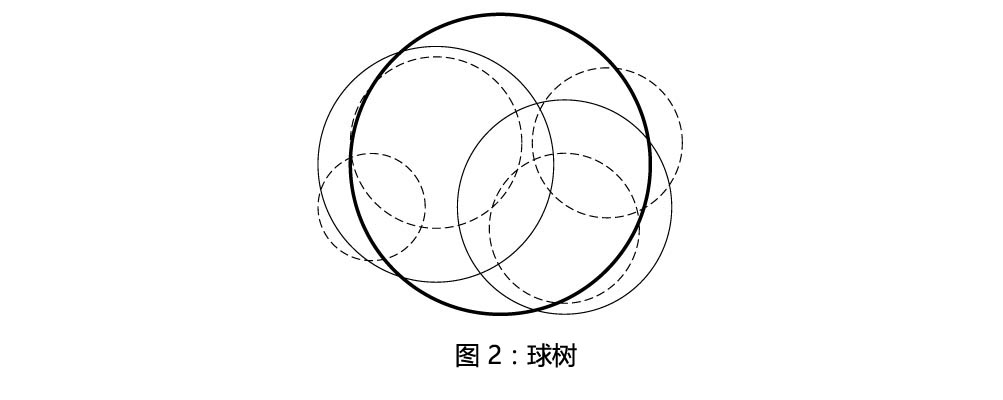
\includegraphics[width=300pt,clip,trim=50 0 0 0]{fig02.jpg}
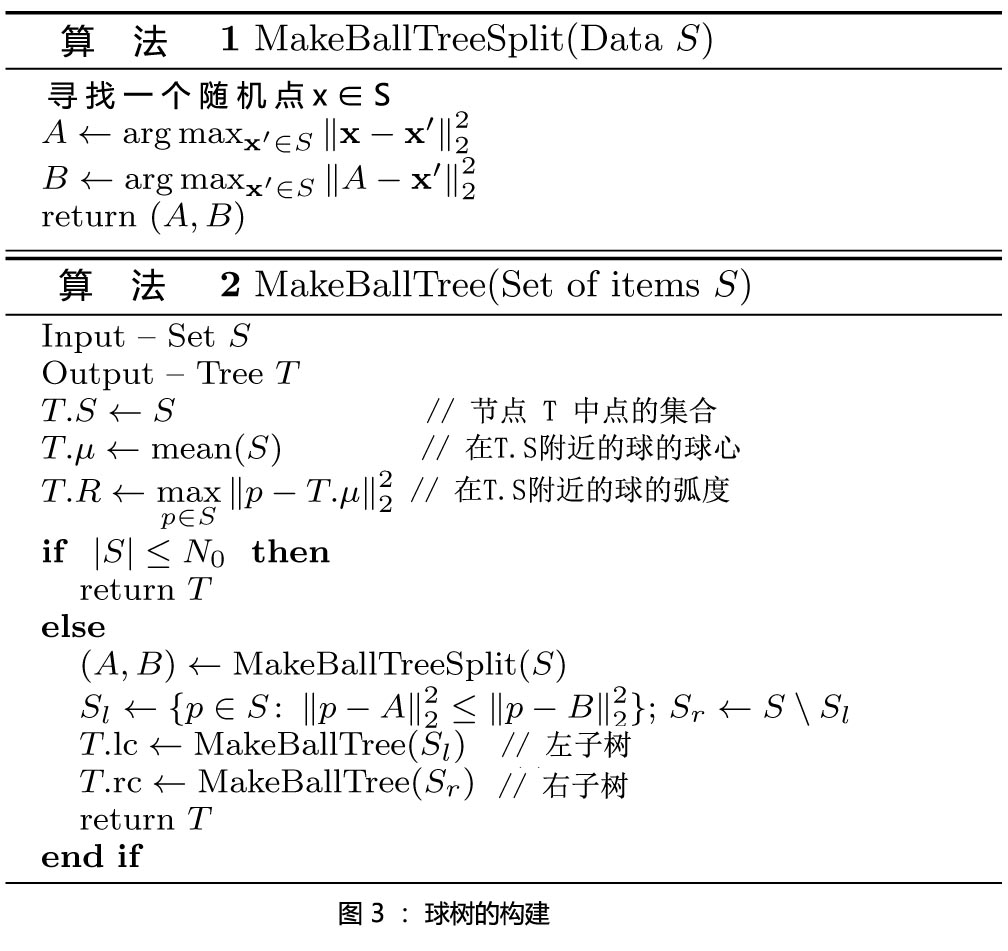
\includegraphics[width=250pt,clip,trim=0 0 0 -30]{fig03.jpg}

\subsection{树的构建}

我们用一个简单的启发式的建树方法 ------ 先近似地选择两个相距最远\cite{28}的主元点,然后通过把点分配给距离它们最近的主元来分割数据。这种启发式背后的直觉在于这些两个点可能位于主方向上。这个基于分割和递归的完整方法在算法1和算法2中给出。

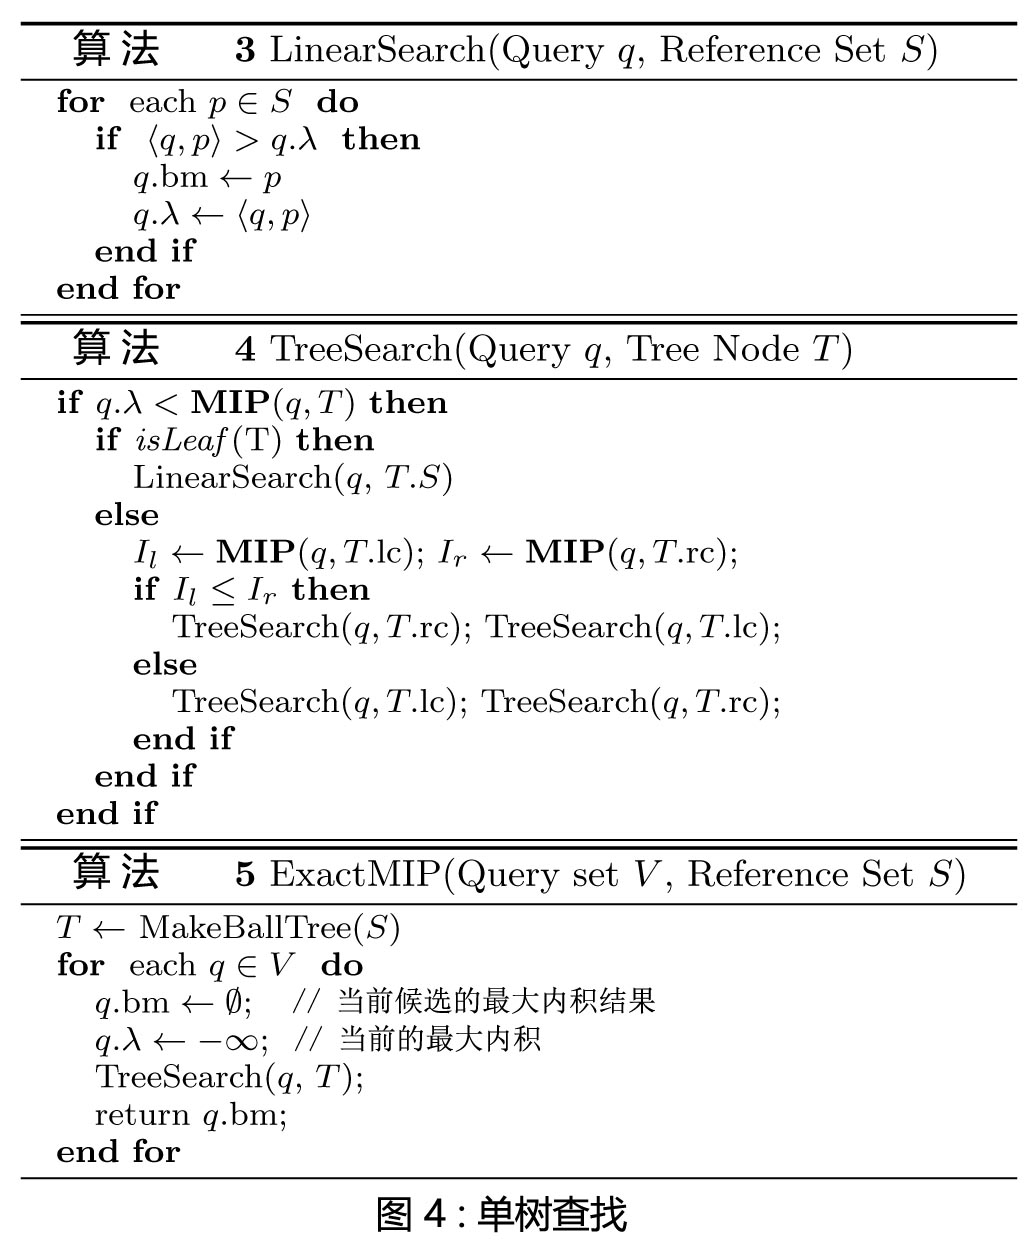
\includegraphics[width=250pt,clip,trim=10 0 0 0]{fig04.jpg}

\subsection{分支定界算法}

球树在最近邻搜索中被广泛地运用,而且它是已知的相对容易被拓展到高维\cite{28, 26}的数据中的数据结构。树的搜索通常会使用深度优先的分支定界算法 ------ 对于一个查询,需要深度优先地遍历这棵树,首先遍历和查询点更接近的点的节点,然后用三角不等式限制住和别的分支可能的最小的距离的界。如果这个到这个分支的最小距离大于到目前的最近邻的距离,那么这个分支就会从计算中被移除。
一个类似的贪心深度优先搜索可以被用与最大内积搜索中,不过对遍历的节点选择会最大化节点中可能存在的点和查询点最大内积,而不是选择遍历和查询点相距更近的节点。递归的分支定界算法在算法4中给出。对于一个查询($q$),算法从树的根部开始(算法 5)。在每一步中,算法都处在一个当前的节点($T$)。检查这个节点中所有的点和查询点的可能的最大内积,$\mathbf{MIP}(q,T)$,是否比当前对于查询的最佳匹配($q.bm$)更好。如果这个检查失败,就不会再去遍历树的这个分支。否则,算法将递归地遍历这棵树,深度优先地查看那些可能会有更好匹配的那些分支。如果这个节点是一个叶子节点,那么算法就只需要在这个节点中线性查找最佳的匹配。这个算法保证在结束时会给出一个精确的解(即最大内积)。

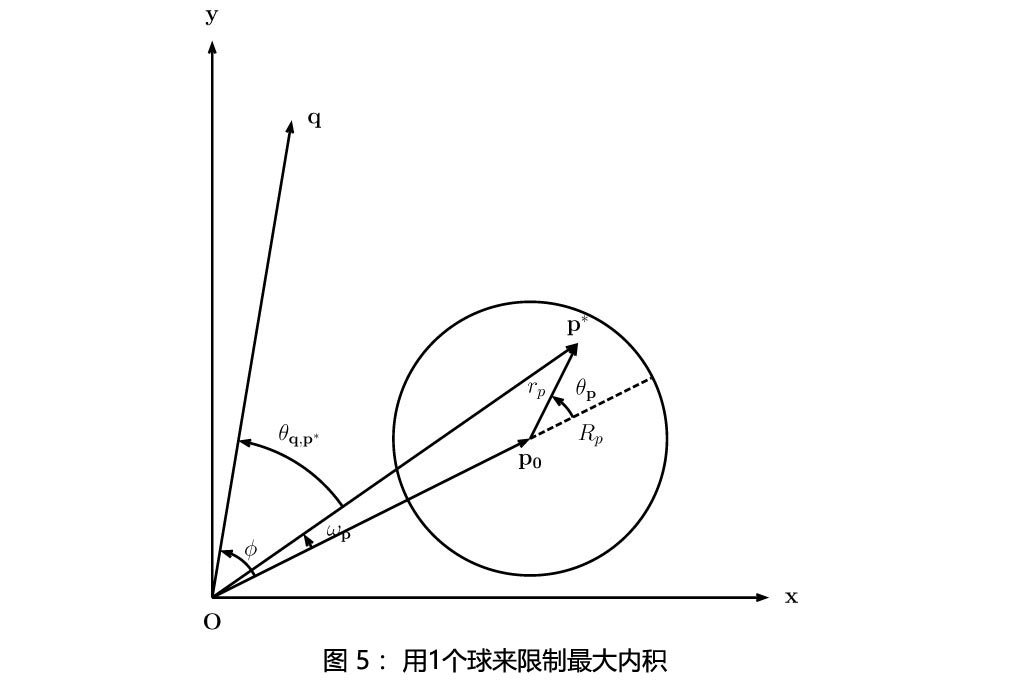
\includegraphics[width=300pt,clip,trim=45 0 0 0]{fig05.jpg}

\subsubsection{用球来限制最大内积}

我们在上面提出了一个新颖方法,来计算一个给定点和球中的点的可能最大内积的解析上界(这个情况下也就是查询$q$)。重要的是要注意,对于一个球的信息被完全限制在它的中心和半径上。在本节剩下的内容中,我们将用$\|\cdot\|$的记号来表示$\|\cdot\|_2$。

\newtheorem{theorem1}{定理}[section]
\begin{theorem1}
给定一个以$p_0$为中心,$R_p$为半径的球$\mathcal{B}_{p_0}^{R_p}$,与一个(查询)点$q$,$q$和球$\mathcal{B}_{p_0}^{R_p}$中点的可能的最大内积的上界为:
\begin{equation}
\max_{p \in \mathcal{B}_{p_0}^{R_p}} \langle q,p \rangle \le \langle q,p_0 \rangle + R_p \|q\|.
\end{equation}

\end{theorem1}
\begin{proof}[证明]
假设对于球$\mathcal{B}_{p_0}^{R_p}$中的查询$q$,$p^*$是可能的最佳匹配点,其中$r_p$为球心$p_0$与$p^*$之间的欧氏距离(根据定义,$r_p \le R_p$)。
令$\theta_p$为向量$\vec{p_0}$与向量$\vec{p_0 p^*}$之间的夹角,$\phi$和$\omega_p$分别为向量$\vec{p_0}$与向量$\vec{q}$,向量$\vec{p^*}$之间的夹角(见图5)。那么$p^*$的长度用$p_0$与$\theta_p$表示也就是:
\begin{equation}
\|p^*\| = \sqrt{(\|p_0\| + r_p\cos\theta_p)^2+(r_p\sin\theta_p)^2}.
\end{equation}
角$\omega_p$可以用$p_0$与$\theta_p$表示成:
\begin{equation}
\cos\omega_p = \frac{\|p_0\|+r_p\cos\theta_p}{\|p^*\|},
\sin\omega_p = \frac{r_p\sin\theta_p}{\|p^*\|}.
\end{equation}
令$\theta_{q,p^*}$为向量$\vec{q}$和$\vec{p*}$间的夹角,根据角之间的三角不等式,我们有:
\begin{equation*}
|\theta_{q,p^*}| \ge |\phi - \omega_p|.
\end{equation*}
假定所有角都在$[-\pi, \pi]$的范围内(而不是通常的$[0, 2\pi]$),我们有:
\begin{equation}
\cos\theta_{q,p^*} \le \cos(\phi - \omega_p).
\end{equation}
用这个不等式我们可以得到下面这个$q$和任意$p \in \mathcal{B}_{p_0}^{R_p}$可能的最大内积的上界
\begin{equation*}
\max_{p \in \mathcal{B}_{p_0}^{R_p}}\langle q,p \rangle = \langle q,p^* \rangle(\mathrm{by\ assumption}) = \|q\|\|p^*\|\cos\theta_{q,p^*}.
\end{equation*}
根据等式4,5,6,我们有:
\begin{align*}
\max_{p \in \mathcal{B}_{p_0}^{R_p}}&\langle q,p \rangle \le \|q\|\|p^*\|\cos(\phi-\omega_p) \\
 &= \|q\|(\cos\phi(\|p_0\|+r_p\cos\theta_p)+\sin\phi(r_p\sin\theta_p))                       \\
 &\le\|q\|\max_{\theta_p}(\cos\phi(\|p_0\| + r_p\cos\theta_p)+\sin\phi(r_p\sin\theta_p))     \\
 &= \|q\|(\cos\phi(\|p_0\|+r_p\cos\phi)+\sin\phi(r_p\sin\phi))                               \\
 &\le \|q\|(\cos\phi(\|p_0\|+R_p\cos\phi)+\sin\phi(R_p\sin\phi)).
\end{align*}
其中,第三个不等式来自最大值的定义。下面的等式来自对$\theta_p$的放大,这就给了我们一个最优的值$\theta_p = \phi$。最后的不等式是因为$r_p \le R_p$的事实。化简最后一个不等式就可以得到不等式3
\end{proof}
对于树的搜索算法(算法4),我们就可以用下面这个式子作为$q$和节点$T$的最大可能内积:
\begin{equation*}
\mathbf{MIP}(q,T) = \langle q,T.\mu\rangle + T.R\|q\|.
\end{equation*}
这个上界几乎可以在要求单个内积的同时计算出来(因为查询的范数可以在做搜索之前就预先计算)。

\section{基于双树的搜索}
对于一组查询,树可以对每个查询分别做一次遍历。然而如果查询点的集合非常的大,那么一个提高查询效率的常见技巧就是把查询也用树来进行索引。这样就可以通过用\emph{双树}算法\cite{15}对两棵树同时进行遍历来进行搜索。
一个基本的想法就是把树遍历的代价均摊到每组类似的查询上。双树算法已经被应用于各种基于树的算法,如最近邻搜索\cite{15},以及核密度估计\cite{16},并且在理论上具有一定的运行效率保证\cite{31}。

\subsection{双树的分枝定界算法}
一个通用的双树算法在算法6中给出。和算法4类似,这个算法向下遍历参考集$S$($RTree$)。而且这个算法也同时向下遍历查询的集合$V$($QTree$),这就形成了一个四路递归。
在每一步,算法在$QTree$的一个节点$Q$以及$RTree$的节点$T$,对于每个$Q$,值$Q.\lambda$代表$Q$中任意一个查询与它当前候选的最佳匹配之间的内积的最小值。如果这个值比任意一个$Q$中的查询和任意一个$T$中的参考点形成可能的最大内积,$\mathbf{MIP}(Q,T)$更大,那么这段递归就不再会继续进行。当这个算法同时处在两个树的叶节点时,它就可以通过对$RTree$叶节点线性扫描来得到$QTree$中每一个查询的最佳匹配。

我们将探索两种对查询进行索引的方式 ------ (1) 用球树来对查询进行索引(算法7中$MakeQueryTree$是算法2)(2)用一个新颖的数据结构锥树来对查询进行索引(算法7中的$MakeQueryTree$是算法9)。在下面的小节中,我们会推导出适用于球树的表达式$\mathbf{MIP}(Q,T)$。适用于锥树的表达式将在第五节中给出。

\subsection{使用球树}
在这个小节中,我们会以下面这个定理给出两个球之间内积的界。
\newtheorem{theorem2}{定理}[section]
\begin{theorem2}
给定两个分别以$p_0$与$q_0$为球心,$R_p$与$R_q$为半径的球$\mathcal{B}_{p_0}^{R_p}$以及$\mathcal{B}_{q_0}^{R_q}$,一对点$p\in\mathcal{B}_{p_0}^{R_p}$和$q\in\mathcal{B}_{q_0}^{R_q}$之间的最大可能内积的上界为:
\begin{equation}
\langle p_0,q_0 \rangle + R_p R_q + \|q_0\|R_p + \|q_0\|R_q.
\end{equation}
\end{theorem2}
\begin{proof}[证明]
考虑一对点$(p^*,q^*),p^*\in\mathcal{B}_{p_0}^{R_p},q^*\in\mathcal{B}_{q_0}^{R_q}$使得:
\begin{equation}
\langle q^*,p^* \rangle = \max_{p^*\in\mathcal{B}_{p_0}^{R_p},q^*\in\mathcal{B}_{q_0}^{R_q}} \langle q,p \rangle.
\end{equation}
令$\theta_p$为$\vec{p_0}$与$\vec{p_0 p^*}$之间的夹角,$\theta_q$为查询球中所对应的角。
令$\omega_p$为$\vec{p_0}$和$\vec{p^*}$之间的夹角,$\omega_q$为$\vec{q_0}$和$\vec{q^*}$之间的夹角。
令$r_p$为$p_0$与$p^*$之间的距离,$r_q$为$q_0$与$q^*$之间的距离。
令$\phi$为$p_0$与$q_0$在原点处的夹角。

对于球$\mathcal{B}_{p_0}^{R_p}$有以下事实(对于球$\mathcal{B}_{q_0}^{R_q}$也类似):
\begin{gather*}
\|p^*\| = \sqrt{\|p_0\|^2+r_p^2+2\|p_0\|r_p\cos\theta_p}, \\
\cos\omega_p = \frac{\|p_0\|+r_p\cos\theta_p}{\|p^*\|},\sin\omega_p = \frac{r_p\sin\theta_p}{\|p^*\|}.
\end{gather*}
根据角之间的三角不等式,我们知道:
\begin{equation*}
|\theta_{q^*,p^*}| \ge |\phi - (\omega_p + \omega_q)|,
\end{equation*}
我们就能得到下面这个等式:
\begin{equation}
\langle q^*,p^* \rangle = \|p^*\|\|q^*\|\cos(\phi-(\omega_p+\omega_q)).
\end{equation}

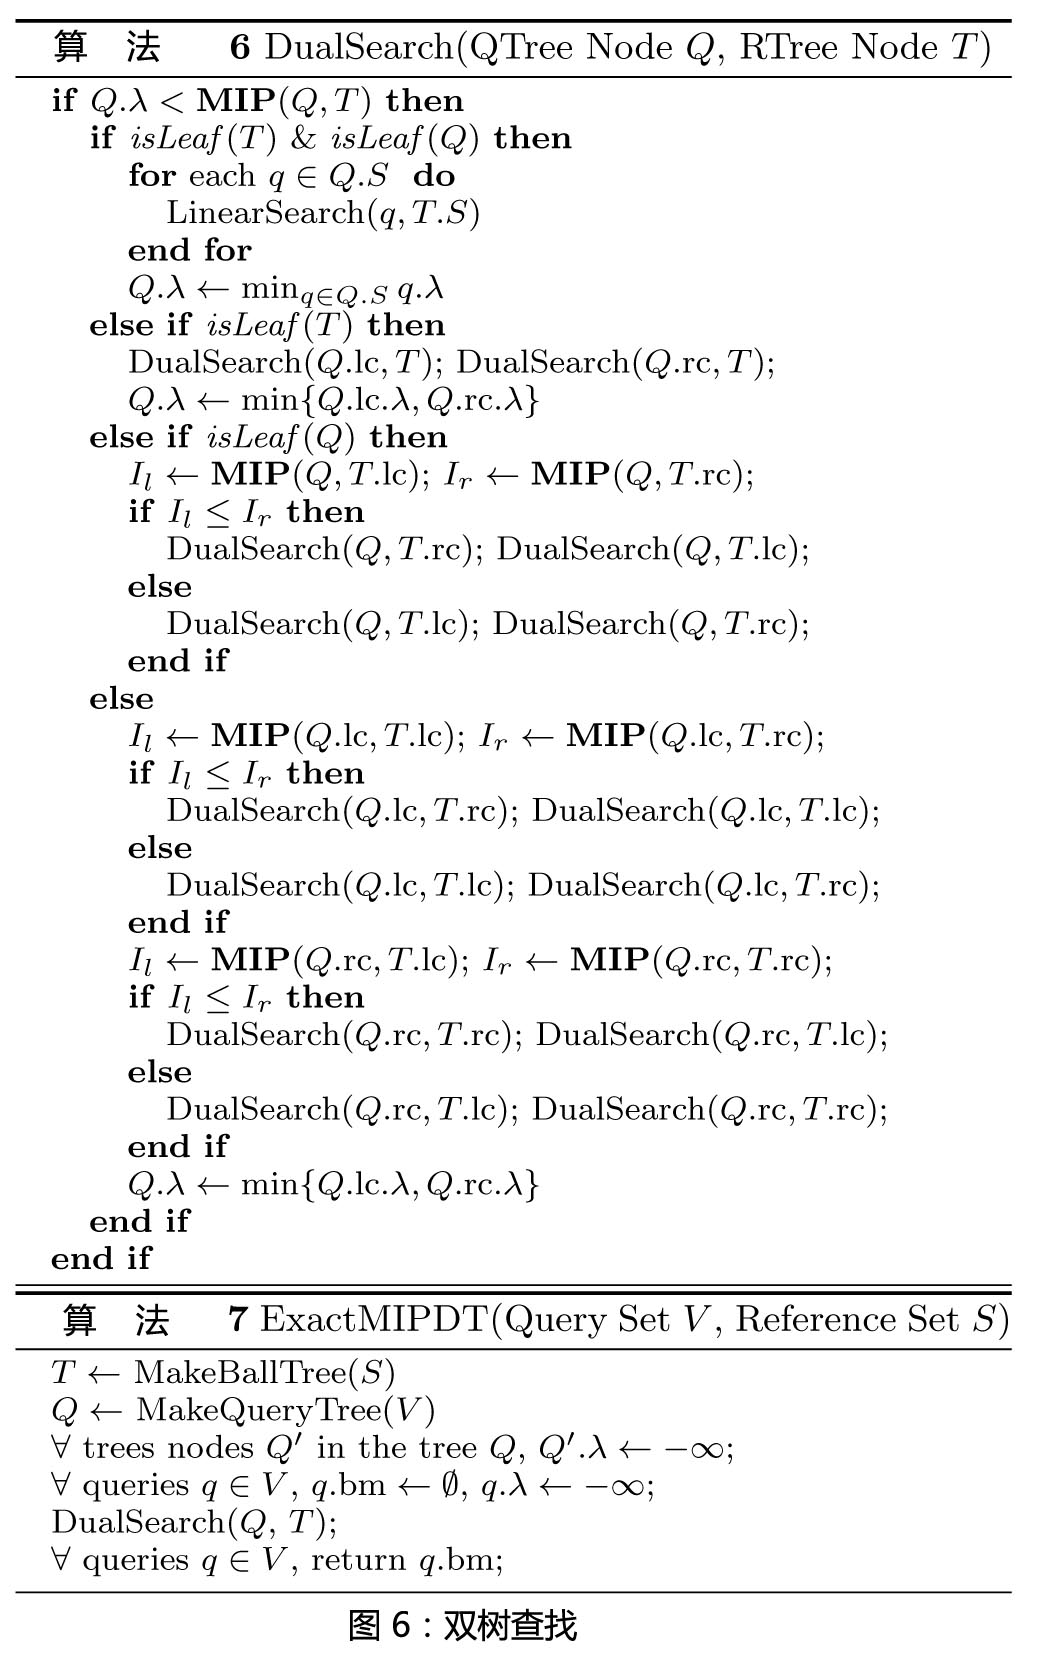
\includegraphics[width=250pt,clip,trim=10 0 0 0]{fig06.jpg}

用$\theta_p$和$\theta_q$来替换上面那个等式中的$\omega_p$和$\omega_q$(和定理3.1的证明类似),我们有:
\begin{align*}
\langle q^*,p^* \rangle =
    & \langle q_0,p_0 \rangle + r_p r_q\cos(\phi-(\omega_p+\omega_q)) \\
    & + r_p\|q_0\|\cos(\phi-\theta_p)+r_q\|p_0\|\cos(\phi-\theta_q) \\
\le & \max_{\theta_p,\theta_q}\langle q_0,p_0 \rangle + r_p r_q\cos(\phi-(\omega_p+\omega_q)) \\
    & + r_p\|q_0\|\cos(\phi-\theta_p)+r_q\|p_0\|\cos(\phi-\theta_q) \\
\le & \max_{\theta_p,\theta_q}\langle q_0,p_0 \rangle + r_p r_q + r_p\|q_0\| + r_q\|p_0\| \\
\le & \langle q_0,p_0 \rangle + R_p R_q + R_p\|q_0\| + R_q\|p_0\|.
\end{align*}
第一个不等式来自对最大值的定义,第二个不等式来自$\cos(\cdot)\le1$,最后一个不等式来自于$r_p \le R_p, r_q \le R_q$的事实
\end{proof}
对于双树的搜索算法(算法6),两棵树的节点$Q$与$T$的最大可能内积为:
\begin{equation*}
\mathbf{MIP}(Q,T)=\langle q_0,p_0 \rangle + R_p R_q + R_q\|p_0\| + R_p\|q_0\|
\end{equation*}
有趣的是,当包含查询点的球中减少至一个点时,也就是$R_q = 0$时,这个上界就退化成定理3.1的上界了。

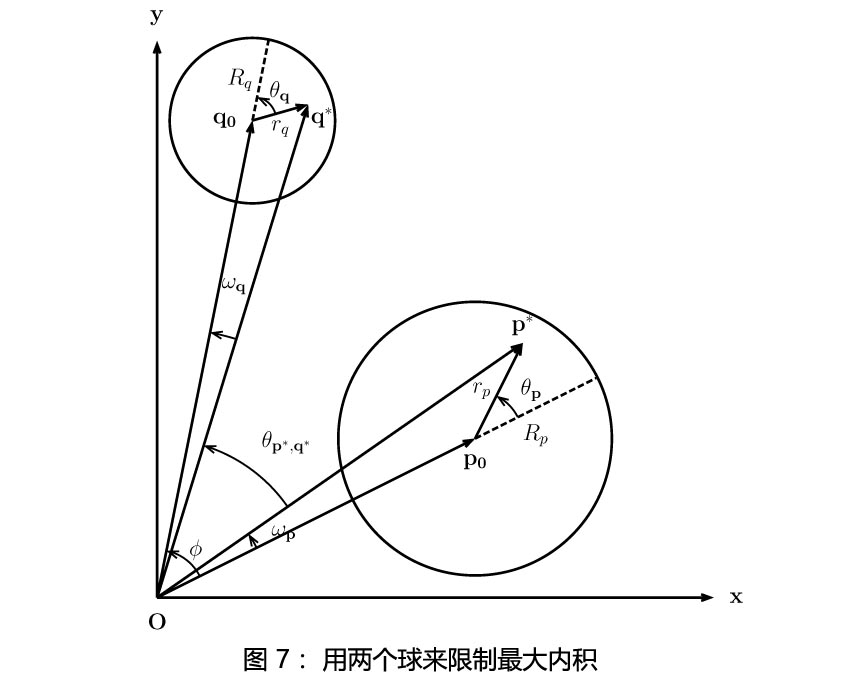
\includegraphics[width=250pt,clip,trim=20 0 0 0]{fig07.jpg}
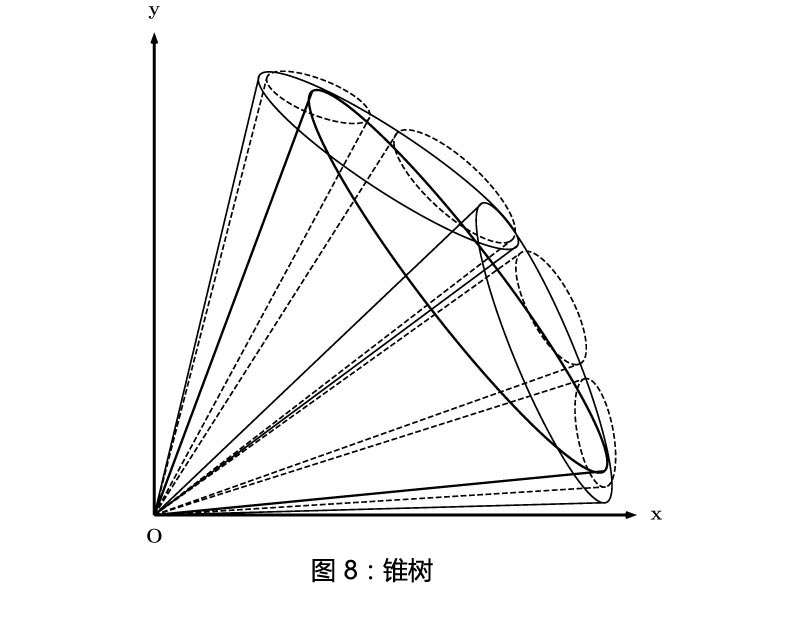
\includegraphics[width=250pt,clip,trim=0 0 0 0]{fig08.jpg}

\section{锥树}
在等式1中,取得内积最大值的点$p$,与查询点$q$的范数$\|q\|$无关。令$\theta_{q,r}$为$q$和$r$在原点处的夹角,那么搜索最大内积的任务也就是找到一个点$p \in S$使得:
\begin{equation}
p = \arg \max_{r \in S}\|r\|\cos\theta_{q,r}
\end{equation}
这也就是说只有查询点的方向会影响结果。每个球提供了内积的一个界是因为它们同时限制了向量的范数和方向。然而因为范数跟查询没有关系,就不需要在球中索引它了(也就是限制它的范数),只有它们的方向的范围需要被限制。基于这个原因,我们提出基于查询点的方向(从原点出发)来对查询进行索引,来形成一个锥树。这些查询点用一些(可能重叠)的开放的锥形来进行分级索引。每个点都表示成向量,对应它们的中轴,以及一个角度,对应它们的孔径
\footnote{一个锥的孔径是中轴和边缘夹角的两倍}。
\subsection{锥树的建立}
锥树的建立和球树的建立十分类似。它们之间唯一的区别就是在分割点时使用了余弦相似度而不是欧氏距离。(详见图8的算法)

\subsection{锥形球的界}
因为查询的范数不会影响等式10中的结果,我们假定所有的查询都具有单位范数。
\newtheorem{theorem3}{定理}[section]
\begin{theorem3}
给定一个以$p_0$为球心,$R_p$为半径的球$\mathcal{B}_{p_0}^{R^p}$与其中的点,已经一个以$q_0$为中轴,孔径$2\omega_q \ge 0$的锥$\mathcal{C}_{q_0}^{\omega_q}$,任意一组点$p\in\mathcal{B}_{p_0}^{R^p},q\in\mathcal{C}_{q_0}^{\omega_q}$之间可能的最大内积的上界为:
\begin{equation}
\|p_0\|\cos(\{|\phi|-\omega_q\}_+)+R_p
\end{equation}
其中$\phi$是$p_0$与$q_0$在原点处的夹角,函数$\{x\}_+ = \max\{x,0\}$。
\end{theorem3}

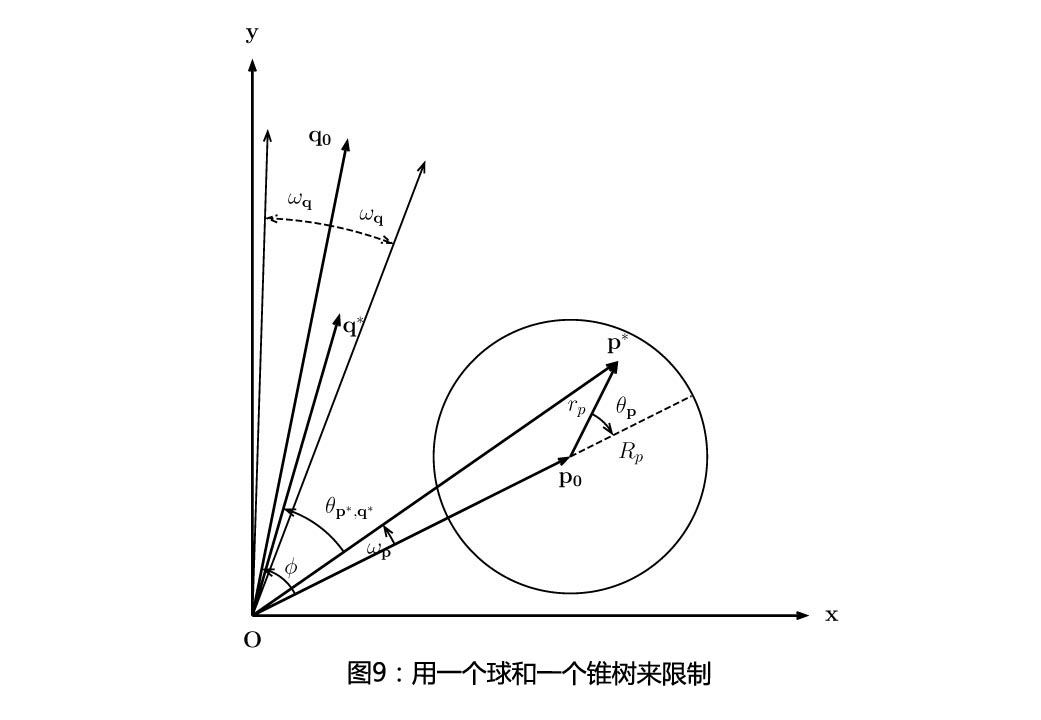
\includegraphics[width=300pt,clip,trim=55 0 0 0]{fig09.jpg}

\begin{proof}[证明]
这里有两种需要考虑的情况:
\begin{enumerate}[label={\roman*}]
\item $|\phi| < \omega_q$
\item $|\phi| \ge \omega_q$
\end{enumerate}
对于情况(i),球$\mathcal{B}_{p_0}^{R^p}$的球心$p_0$在锥$\mathcal{C}_{q_0}^{\omega_q}$之内,也就是说:
\begin{equation}
\max_{q\in\mathcal{C}_{q_0}^{\omega_q},p\in\mathcal{B}_{p_0}^{R_p}}\|p\|\cos\theta_{q,p} \le \|p_0\| + R_p
\end{equation}
因为有一些查询$q^*\in\mathcal{C}_{q_0}^{\omega_q}$和$p_0$的方向相同,就直接给出最大的可能内积。

对于情况(ii),我们假定$\phi\ge0$不会丧失这个问题的一般性。那么$\phi\ge\omega_q$。继续使用定理3.1和4.1中表达最佳的点对$(q^*,p^*)$,以及图9中的记号,我们可以说:
\begin{equation}
|\theta_{p^*,q^*}| \ge | \phi - \omega_q - \omega_p |
\end{equation}
因为$\omega_q$是固定的,我们就可以继续说:
\begin{equation}
\begin{aligned}
\max_{q\in\mathcal{C}_{q_0}^{\omega_q},p\in\mathcal{B}_{p_0}^{R_p}} \|p\|\cos\theta_{q,p} & \le \|p^*\|\cos\theta_{q^*,p^*}\text{(by def)} \\
& \le \|p^*\|\cos(\phi - \omega_q - \omega_p).
\end{aligned}
\end{equation}

用$\|p_0\|$,$r_p$和$\theta_p$来表示$\|p^*\|$和$\omega_p$,接下来最大化$\theta_p$,用$r_p \le R_p$这些事实,我们可以得到:
\begin{equation}
\max_{q\in\mathcal{C}_{q_0}^{\omega_q},p\in\mathcal{B}_{p_0}^{R_p}} \|p\|\cos\theta_{q,p} \le \|p_0\|\cos(\phi - \omega_q) + R_p
\end{equation}
把情况(i)和(ii)结合起来,我们就得到了式11。
\end{proof}

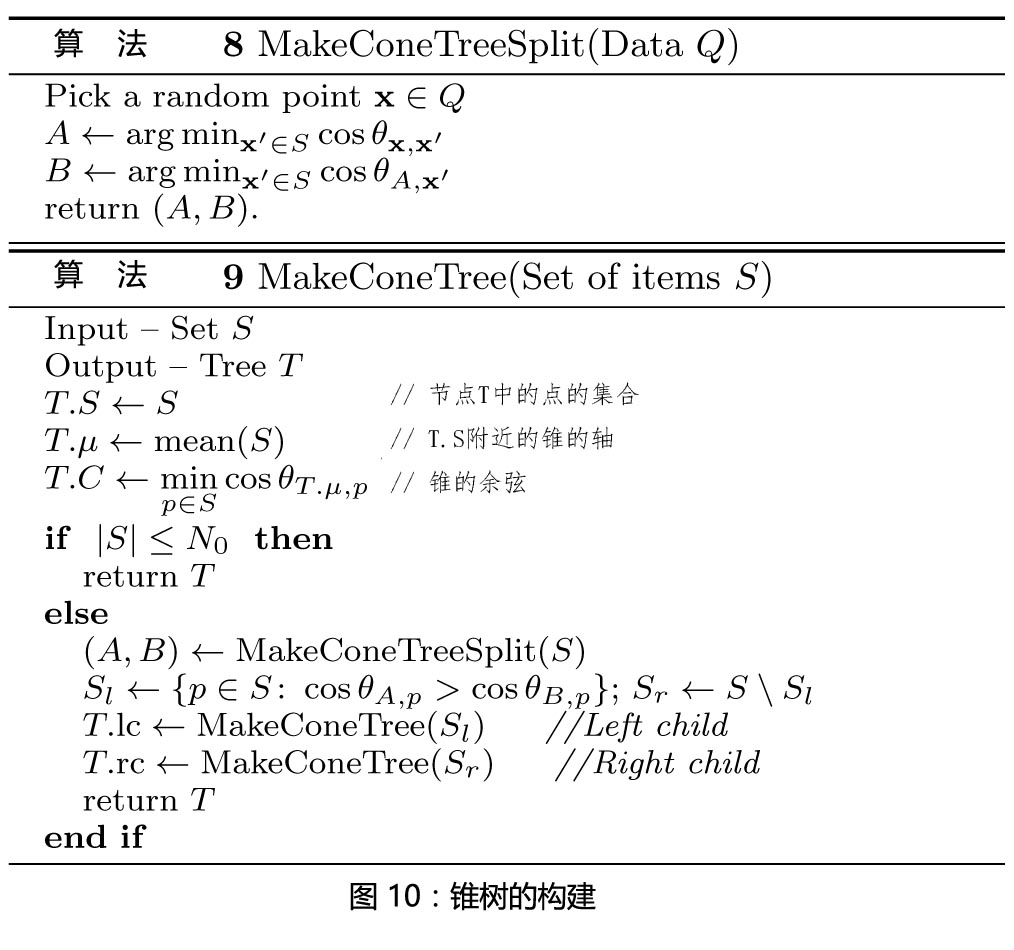
\includegraphics[width=250pt,clip,trim=10 0 -10 0]{fig10.jpg}

\begin{table}[]
\centering
\begin{tabular}{|c|c|c|c|}
\hline
Dataset     & Dimensions & Reference set & Query Set \\
\hline
Bio         & 74         & 210,409       & 75,000    \\
\hline
Corel       & 32         & 27,749        & 10,000    \\
\hline
Covertype   & 55         & 431,012       & 150,000   \\
\hline
LCDM        & 3          & 10,777,216    & 6,000,000 \\
\hline
LiveJournal & 25,327     & 121,625       & 100,000   \\
\hline
MNIST       & 786        & 60,000        & 10,000    \\
\hline
MovieLens   & 51         & 3,706         & 6,040     \\
\hline
Netflix     & 51         & 17,770        & 480,189   \\
\hline
OptDigits   & 64         & 1,347         & 450       \\
\hline
Pall7       & 7          & 100,841       & 100,841   \\
\hline
Physics     & 78         & 112,500       & 37,500    \\
\hline
PSF         & 2          & 3,056,092     & 3,056,092 \\
\hline
SJ2         & 2          & 50,000        & 50,000    \\
\hline
U-Random    & 20         & 700,000       & 300,000   \\
\hline
Y!-Music    & 51         & 624,961       & 1,000,990 \\
\hline
\end{tabular}
\caption{用于评估的数据集}
\label{table1}
\end{table}

\section{实验与结果}
在这一节,我们将对算法5(SB - Single Ball Tree)和算法7的效率进行评估。对于双树的算法,我们用了它的两个变体 --
\begin{enumerate*}[label={\roman*}]
\item 用球树来索引查询点(DBB -- Dual ball-ball)
\item 用锥树来索引查询点(DBC -- Dual ball-cone)
\end{enumerate*}。
我们把我们提出的算法和在算法3中给出的线性搜索(LS -- linear search)进行了比较。我们将报告我们的算法相对于线性搜索的加速比
\footnote{加速比被定义为是线性搜索使用的时间和被评估的算法所使用的时间的比值}。
对于树来说,叶子中含有点的数量$N_0$可以通过交叉验证的方式来选择,不过我们对所有的数据集专门选了一个值,$N_0 = 20$,来说明用我们的算法得到的效率的提升不需要任何复杂的交叉验证。

\paragraph{数据集}
我们使用了各种来自不同的数据挖掘的领域的数据集。我们用了以下合作公司的数据集:MovieLens\cite{17},Netflix\cite{3}和Yahoo! Music\cite{12}数据集。对于文本数据,我们使用了LiveJournal Blog moods数据集\cite{19}。我们同样使用了MNIST digits数据集\cite{24}来做评估。我们同样考虑了三个天文方面的数据集,LCDM\cite{27},PSF和SJ2。我们还用了一个用20维随机分布的点合成数据集(U-Rand)\cite{5}。其他数据集都是在机器学习中被广泛运用的,来自UCI机器学习仓库。数据集的细节由表1给出
\footnote{对于合作筛选的数据集,参考点(项目)和查询(用户)是被明确定义的,我们随机地从数据集中选出查询集($V$),剩下的作为参考集($S$)}。

\paragraph{建树时间}
建树的效率是非常高的。我们在表6中给出了建树时间并把他们和线性搜索的运行时间进行了对比。在最后一列中,我们展示了建树时间和算法3中运行时间的对比。对于单个球和两个球的树算法,建树中分别包括了构造一个和两个球树。对于“dual ball-cone”的算法,为了方便起见,所有查询都被标准化为单位长度
\footnote{这是因为查询点的范数不会影响结果}。
在标准化查询之后,会建立两个树。标准化查询的时间被要求包括在建树的时间中,这就使“dual ball-ball”和“dual ball-cone”算法的建树时间有显著的差别。

表6(R)最后一列的数字告诉我们建树时间相对于真正线性查找的运行时间是有多小。最高的比例只有OptDigits数据集的0.15。这就代表查找时只要比线性查找快1.18倍就可以弥补建树的代价。对于更多的数据集,这个比例还要更小。而且,建树的代价只有一次。当一棵树已经建好之后,它就可以多次地被用作查询。

\begin{table}[]
\centering
\begin{tabular}{|c|c|c|c|}
\hline
Dataset     & Dimensions & Reference set & Query Set \\
\hline
Bio         & 74         & 210,409       & 75,000    \\
\hline
Corel       & 32         & 27,749        & 10,000    \\
\hline
Covertype   & 55         & 431,012       & 150,000   \\
\hline
LCDM        & 3          & 10,777,216    & 6,000,000 \\
\hline
LiveJournal & 25,327     & 121,625       & 100,000   \\
\hline
MNIST       & 786        & 60,000        & 10,000    \\
\hline
MovieLens   & 51         & 3,706         & 6,040     \\
\hline
Netflix     & 51         & 17,770        & 480,189   \\
\hline
OptDigits   & 64         & 1,347         & 450       \\
\hline
Pall7       & 7          & 100,841       & 100,841   \\
\hline
Physics     & 78         & 112,500       & 37,500    \\
\hline
PSF         & 2          & 3,056,092     & 3,056,092 \\
\hline
SJ2         & 2          & 50,000        & 50,000    \\
\hline
U-Random    & 20         & 700,000       & 300,000   \\
\hline
Y!-Music    & 51         & 624,961       & 1,000,990 \\
\hline
\end{tabular}
\caption{树的建立时间(秒)与线性搜索的时间(秒)的对比}
\label{table2}
\end{table}

\paragraph{查找效率}
相对于线性查找,查找效率的提升在表6中给出。总体来说,加速比从低至OptDigits的1.13到LCDM和PSF数据集的$10^5$(4个数量级)那么多。重要的是,需要注意所有加速比很低的(比一个数量级还小)使用单个球的算法,三个算法的加速比都十分低,相对还是具有可比性的。然而,甚至加速比达到2了之后对于绝对的速度提升也是十分显著的。比如对于Yahoo!Music数据集,2的加速比加上120秒的建树时间节省了总共19小时的计算时间。对于绝大多数对于单个球的算法具有很高加速比的数据集,双树算法的加速比也非常高。

\begin{table}[]
\centering
\begin{tabular}{|c|c|c|c|}
\hline
Dataset     & Dimensions & Reference set & Query Set \\
\hline
Bio         & 74         & 210,409       & 75,000    \\
\hline
Corel       & 32         & 27,749        & 10,000    \\
\hline
Covertype   & 55         & 431,012       & 150,000   \\
\hline
LCDM        & 3          & 10,777,216    & 6,000,000 \\
\hline
LiveJournal & 25,327     & 121,625       & 100,000   \\
\hline
MNIST       & 786        & 60,000        & 10,000    \\
\hline
MovieLens   & 51         & 3,706         & 6,040     \\
\hline
Netflix     & 51         & 17,770        & 480,189   \\
\hline
OptDigits   & 64         & 1,347         & 450       \\
\hline
Pall7       & 7          & 100,841       & 100,841   \\
\hline
Physics     & 78         & 112,500       & 37,500    \\
\hline
PSF         & 2          & 3,056,092     & 3,056,092 \\
\hline
SJ2         & 2          & 50,000        & 50,000    \\
\hline
U-Random    & 20         & 700,000       & 300,000   \\
\hline
Y!-Music    & 51         & 624,961       & 1,000,990 \\
\hline
\end{tabular}
\caption{与线性搜索相比的速度倍数}
\label{my-label}
\end{table}

还有三件非常重要的事需要注意。首先,如单个树的算法(算法5)加速比不高的话,双树算法(算法7)也不会有特别好的表现。这很大程度上是因为树无法找到非常严格的界,所以需要遍历非常多的分支。双树的算法放松了界限来把遍历的代价均摊到每个查询上。但是如果这个界对于算法5来说比较差,对于双树的界就会更差。因此,双树算法没有表现出任何显著的速度提升。
第二,当查询的数据集数量非常大的时候,双树算法(尤其是“dual ball-cone”算法)就开始显著地单个树算法更优秀。这对于双树算法来说是一个很普遍的状况。查询集一定要足够大,才能使遍历参考树的效率均摊到查询上之后,超过遍历查询树本身的开销。
最后,在一般情况下,使用球树的双树算法会显著地比使用锥树来做查询要更慢。这很可能是因为这两个原因 --
\begin{enumerate*}[label={\roman*}]
\item 锥形对于查询提供了一个更紧密的索引,单个锥就可以索引很多个方向相近但是范数不同的球。
\item 等式10中的$\mathbf{MIP}(Q,T)$是相当松的一个上界。
\end{enumerate*}。

我们同样考虑了一个更一般的问题,也就是对于查询$q$检索在集合$S$中第$k$大的内积的点。这和第$k$近邻搜索问题十分类似,我们同样对我们的算法在图11中给出了当$k$ = 1,2,5和10时,相对于线性查找的加速比。

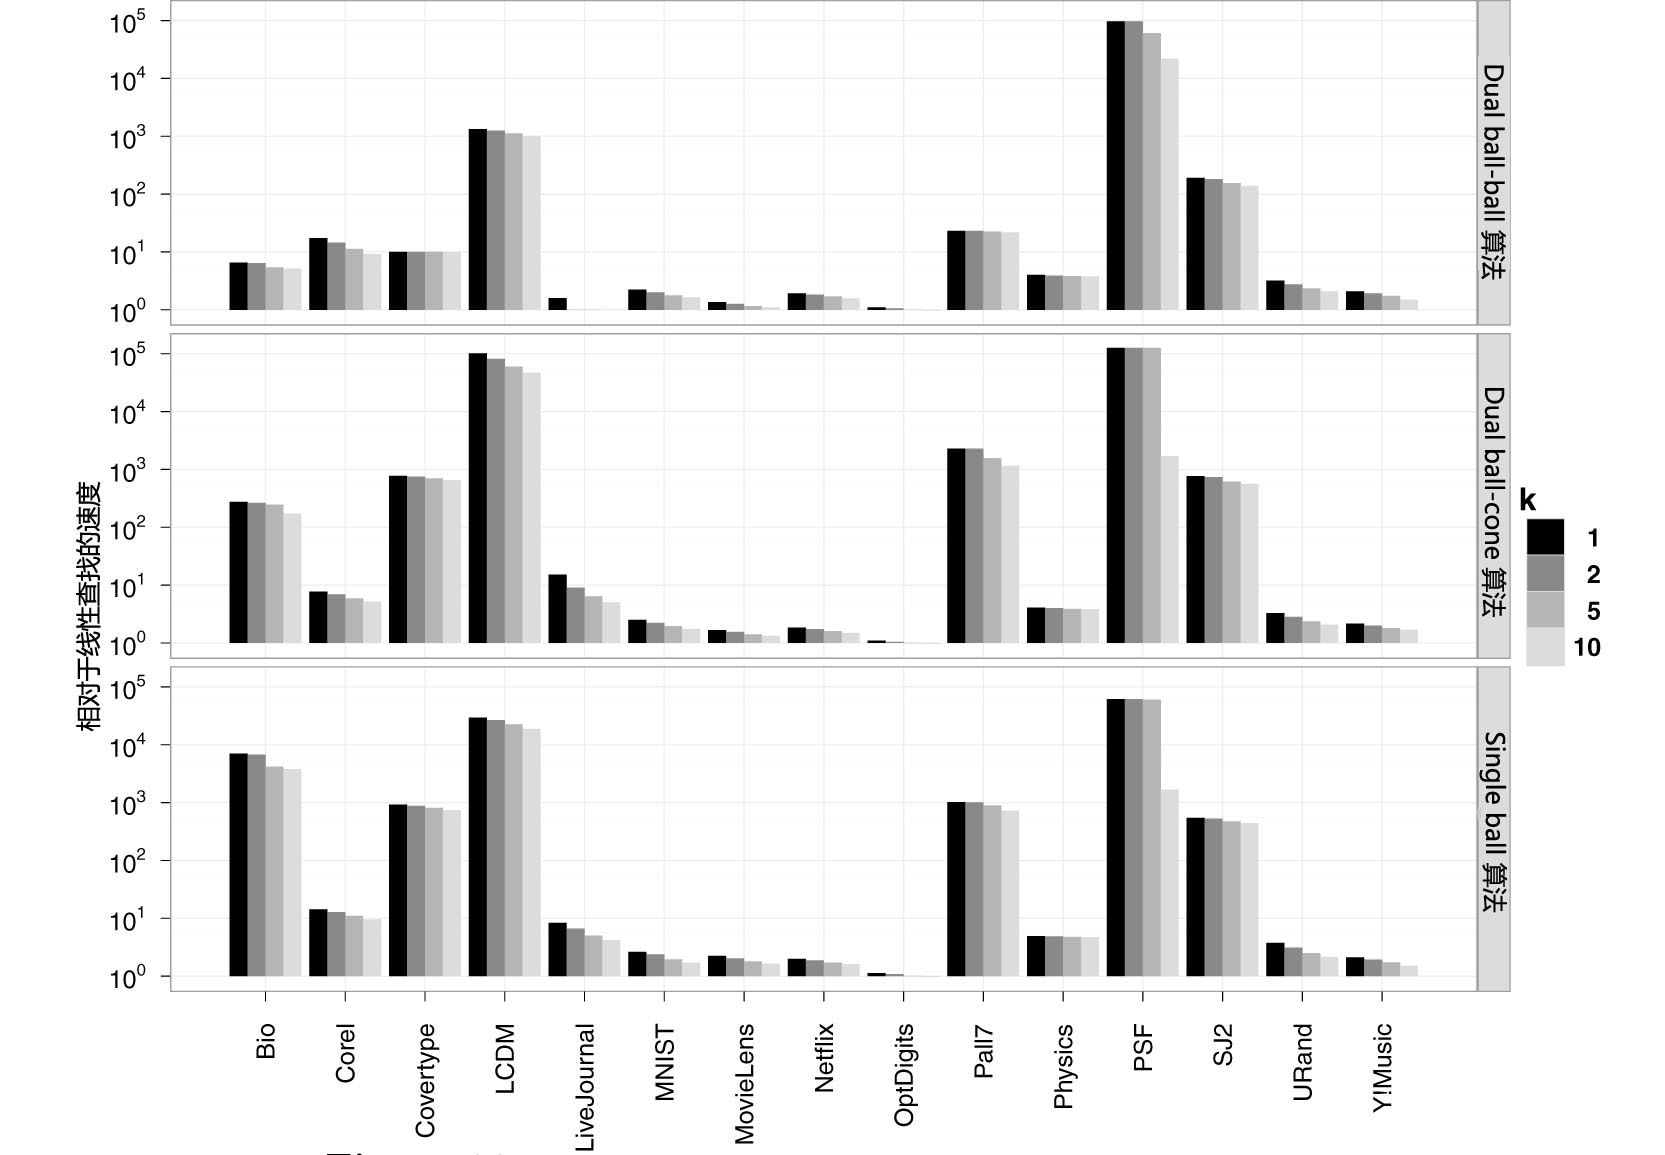
\includegraphics[width=250pt,clip,trim=0 0 0 0]{fig11.jpg}

\section{最大核操作和一般的核函数}
在这一节中,我们提供了一些讨论,关于如何在不显式地把点表示成内积空间中的条件下,把前面提出的那些算法应用到一个内积空间中。内积的定义是一个核函数$\mathcal{K}(q,p)=\langle \varphi(q),\varphi(p) \rangle.$

要在内积空间中做这件事,我们就要修改一下建树的过程。对于一个节点$T$和它的点集$T.S$,在$\varphi$-空间中的均值被定义为$\mu=\frac{1}{|T.S|}\sum_{p\in T.S}\varphi(p)$。然而,$\mu$不一定有一个显式的表示形式,但是有可能用下面的方法计算出与$\mu$的内积:
\begin{equation*}
\langle\mu,\varphi(q)\rangle = \frac{1}{|T.S|}\sum_{p \in T.S}\mathcal{K}(q,p).
\end{equation*}
然而计算这个式子的开销在搜索过程中可能就会显得非常大。因此我们认为,选择一个在$\varphi$-空间中,最接近均值$\mu$的那个点当做新的球心。所以新的球心$p_c$可以这样给出:
\begin{equation}
p_c = \arg\min_{r\in T.S}\mathcal{K}(r,r) - \frac{2}{T.S}\sum_{r'\in T.S}\mathcal{K}(r',r).
\end{equation}
这个操作在计算上是二次的,不过可以在预处理阶段做这件事来获得查询阶段效率的提升。对于一个球心$p_c$,包围住$\varphi$-空间中的点集$T.S$的球的半径$R_p$可以由下式给出:
\begin{equation}
R_p^2 = \max_{r\in T.S}\mathcal{K}(p_c,p_c)+\mathcal{K}(r,r) - 2\mathcal{K}(r,p_c)
\end{equation}
由这些对于球心和半径的定义,一个球树用算法2在任意的$\varphi$-空间中建立。给定一个$\varphi$空间中的球,定理3.1中的等式3就变为:
\begin{equation}
\mathbf{MIP}(q,T) = \mathcal{K}(q,p_c) + R_p\sqrt{\mathcal{K}(q,q)}.
\end{equation}
这个上界的计算等价于单个核函数的求值($\mathcal{K}(q,q)$可以在搜索之前提前计算出来)。用这个上界,树的搜索算法(算法5)就可以在任意的$\varphi$空间进行。我们在这篇论文一个较长的版本中对这个算法进行评估。

用同样的原则,双树的算法(算法7)也可以被应用到任意的$\varphi$空间中。对于使用球树来进行查询的双树,定理4.1中查询节点Q和节点T的最大可能内积的上界可以被修改成:
\begin{equation}
\mathcal{K}(q_c, p_c) + R_p R_q + R_q \sqrt{\mathcal{K}(q_c,q_c)} + R_q \sqrt{\mathcal{K}(p_c, p_c)}
\end{equation}
其中$p_c$和$q_c$是在$\varphi$-空间中的球心,它们的半径分别为$R_p$和$R_q$

对于使用锥树进行索引的查询,在$\varphi$-空间中,锥的中轴点可以被选为和$\varphi$-空间的均值夹角最小的点。因为在$\varphi$-空间中的查询也应当被标准化,对于一个查询树的节点$Q$,集合$Q.S$的均值应当为$\mu=\frac{1}{Q.S}\sum_{q \in Q.S}\frac{\varphi(q)}{\|\varphi(q)\|}$,所以新的锥中轴点$q_c$为:
\begin{equation}
q_c = \arg \max_{q\in Q.S}\frac{\sum_{q'\in Q.S}\frac{\mathcal{K}(q',q)}{\sqrt{\mathcal{K}(q',q')}}}{\mathcal{K}(r,r)}
\end{equation}
同样,这个计算时间对于数据集的大小来说是二次的,但是可以给搜索时间提高效率。半孔径的余弦值为:
\begin{equation}
\cos\omega_q = \min_{q \in Q.S}\frac{\mathcal{K}(q_c, q)}{\sqrt{\mathcal{K}(q_c, q_c)\mathcal{K}(q,q)}}
\end{equation}
定理5.1对于锥树查询节点Q和球树参考节点T的上界就变为:
\begin{equation}
\sqrt{\mathcal{K}(p_c, p_c)}\cos(\{|\phi| - \omega_q\}_+) + R_p
\end{equation}
其中$\phi$的定义为:
\begin{equation*}
\cos\phi = \frac{\mathcal{K}(p_c, q_c)}{\sqrt{\mathcal{K}(q_c, q_c)\mathcal{K}(p_c,p_c)}}
\end{equation*}
这个界的计算效率是很高的,是因为他只需要一个核函数的求值($\mathcal{K}(q_c, q_c)$和$\mathcal{K}(p_c,p_c)$两项可以被提前计算出来并且保存在树中)。

\section{结论}

我们考虑了一般的最大内积搜索的问题,而且用几个新颖的基于树的方法高效地解决了这个问题。我们用树形结构,并且用了“branch-and-bound”算法来进行最大内积搜索。我们还展示了一个双树算法来应对多个请求的状况。我们用了各种的数据集,对我们的算法进行了评估,并且展现出算法在计算上的效率。

对于我们的算法一个理论上的分析会让我们更好地理解这些算法的效率。对我们算法运行时间进行严格的分析是我们未来在这个方向工作的一部分。

\section{参考文献}
\renewcommand{\section}[2]{}
\begin{thebibliography}{1}
\bibitem{1} R. Bayardo, Y. Ma, and R. Srikant. Scaling Up All Pairs Similarity Search. \emph{In Proceedings of the 16th Intl. Conf. on World Wide Web}, 2007.
\bibitem{2} R. M. Bell and Y. Koren. Lessons from the Netflix Prize Challenge. \emph{SIGKDD Explor. Newsl.}, 2007.
\bibitem{3} J. Bennett and S. Lanning. The Netflix Prize. In \emph{Proc. KDD Cup and Workshop}, 2007.
\bibitem{4} A. Beygelzimer, S. Kakade, and J. Langford. Cover Trees for Nearest Neighbor. \emph{Proceedings of the 23rd Intl. Conf. on Machine Learning}, 2006.
\bibitem{5} C. L. Blake and C. J. Merz. UCI Machine Learning Repository. http://archive.ics.uci.edu/ml/, 1998.
\bibitem{6} L. Cayton and S. Dasgupta. A Learning Framework for Nearest Neighbor Search. \emph{Advances in Neural Info. Proc. Systems 20}, 2007.
\bibitem{7} M. S. Charikar. Similarity Estimation Techniques from Rounding Algorithms. In \emph{Proceedings of the 34th
annual ACM Symp. on Theory of Comp.}, 2002.
\bibitem{8} P. Ciaccia and M. Patella. PAC Nearest Neighbor Queries: Approximate and Controlled Search in High-dimensional and Metric spaces. \emph{Proceedings of 16th Intl. Conf. on Data Engineering}, 2000.
\bibitem{9} K. Clarkson. Nearest-neighbor Searching and Metric Space Dimensions. \emph{Nearest-Neighbor Methods for
Learning and Vision: Theory and Practice}, 2006.
\bibitem{10} S. Dasgupta and Y. Freund. Random projection trees and low dimensional manifolds. In \emph{Proceedings of the
40th annual ACM Symp. on Theory of Comp.}, 2008.
\bibitem{11} S. C. Deerwester, S. T. Dumais, T. K. Landauer, G. W. Furnas, and R. A. Harshman. Indexing by Latent Semantic Analysis. \emph{Journal of the American Society of Info. Science}, 1990.
\bibitem{12} G. Dror, N. Koenigstein, Y. Koren, and M. Weimer. The Yahoo! Music Dataset and KDD-Cup’11. \emph{Journal Of Machine Learning Research}, 2011.
\bibitem{13} J. H. Freidman, J. L. Bentley, and R. A. Finkel. An Algorithm for Finding Best Matches in Logarithmic Expected Time. \emph{ACM Trans. Math. Softw.}, 1977.
\bibitem{14} A. Gionis, P. Indyk, and R. Motwani. Similarity Search in High Dimensions via Hashing. \emph{Proceedings of the 25th Intl. Conf. on Very Large Data Bases}, 1999.
\bibitem{15} A. G. Gray and A. W. Moore. ‘N -Body’ Problems in Statistical Learning. In \emph{Advances in Neural Info. Proc. Systems 13}, 2000.
\bibitem{16} A. G. Gray and A. W. Moore. Nonparametric Density Estimation: Toward Computational Tractability. In \emph{SIAM Data Mining}, 2003.
\bibitem{17} GroupLens. MovieLens dataset.
\bibitem{18} P. Indyk and R. Motwani. Approximate Nearest Neighbors: Towards Removing the Curse of Dimensionality. In \emph{Proceedings of the 30th annual ACM Symp. on Theory of Comp.}, 1998.
\bibitem{19} S. Kim, F. Li, G. Lebanon, and I. Essa. Beyond Sentiment: The Manifold of Human Emotions. \emph{Arxiv preprint arXiv:1202.1568}, 2011.
\bibitem{20} M. Klaas, D. Lang, and N. de Freitas. Fast Maximum-a-posteriori Inference in Monte Carlo State Spaces. In \emph{Artificial Intelligence and Statistics}, 2005.
\bibitem{21} Y. Koren. The BellKor solution to the Netflix Grand Prize. 2009.
\bibitem{22} Y. Koren, R. M. Bell, and C. Volinsky. Matrix Factorization Techniques for Recommender Systems. \emph{IEEE Computer}, 2009.
\bibitem{23} B. Kulis and K. Grauman. Kernelized Locality-sensitive Hashing for Scalable Image Search.  In \emph{IEEE 12th Intl. Conf. on Computer Vision}, 2009.
\bibitem{24} Y. LeCun. MNist dataset, 2000. http://yann.lecun.com/exdb/mnist/.
\bibitem{25} Z. Li, H. Ning, L. Cao, T. Zhang, Y. Gong, and T. S. Huang. Learning to Search Efficiently in High Dimensions. In \emph{Advances in Neural Info. Proc. Systems 24}. 2011.
\bibitem{26} T. Liu, A. W. Moore, A. G. Gray, and K. Yang. An Investigation of Practical Approximate Nearest Neighbor Algorithms. In \emph{Advances in Neural Info. Proc. Systems 17}, 2005.
\bibitem{27} R. Lupton, J. Gunn, Z. Ivezic, G. Knapp, S. Kent, and N. Yasuda. The SDSS Imaging Pipelines. \emph{Arxiv preprint astro-ph/0101420}, 2001.
\bibitem{28} S. M. Omohundro. Five Balltree Construction Algorithms. Technical report, International Computer Science Institute, December 1989.
\bibitem{29} F. P. Preparata and M. I. Shamos. \emph{Computational Geometry: An Introduction}. Springer, 1985.
\bibitem{30} A. Rahimi and B. Recht. Random Features for Large-scale Kernel Machines. \emph{Advances in Neural Info. Proc. Systems 20}, 2007.
\bibitem{31} P. Ram, D. Lee, W. March, and A. Gray. Linear-time Algorithms for Pairwise Statistical Problems. In \emph{Advances in Neural Info. Proc. Systems 22}. 2009.
\bibitem{32} P. Ram, D. Lee, H. Ouyang, and A. G. Gray. Rank-Approximate Nearest Neighbor Search: Retaining Meaning and Speed in High Dimensions. In \emph{Advances in Neural Info. Proc. Systems 22}. 2009.
\end{thebibliography}

\end{document}
